\section{Hauptteil}

\begin{frame}{Hauptteil}
$$
\begin{aligned}
    \nabla \times \vec{\mathbf{B}} -\, \frac1c\, \frac{\partial\vec{\mathbf{E}}}{\partial t} & = \frac{4\pi}{c}\vec{\mathbf{j}} \\   \nabla \cdot \vec{\mathbf{E}} & = 4 \pi \rho \\
    \nabla \times \vec{\mathbf{E}}\, +\, \frac1c\, \frac{\partial\vec{\mathbf{B}}}{\partial t} & = \vec{\mathbf{0}} \\
    \nabla \cdot \vec{\mathbf{B}} & = 0
\end{aligned}
$$
\end{frame}

% http://en.wikibooks.org/wiki/LaTeX/Presentations#Blocks
\begin{frame}{Example of columns 2}
     \begin{columns}[T]
        % contents are top vertically aligned
         \begin{column}[T]{5cm}
            % each column can also be its own environment
            \lipsum[66]
         \end{column}
         \begin{column}[T]{5cm}
            % alternative top-align that's better for graphics
            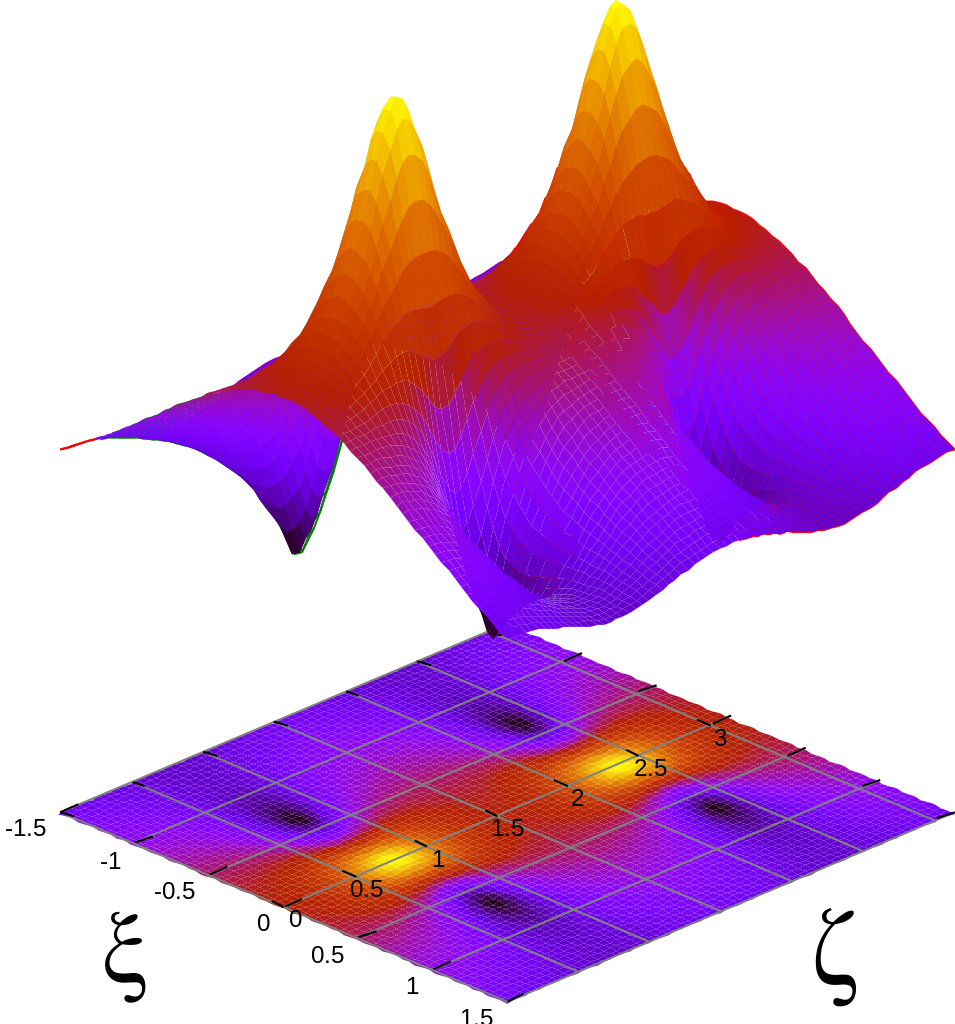
\includegraphics[width=\textwidth]{resources/plot.png}
         \end{column}
     \end{columns}
\end{frame}